\def\year{2021}\relax
%File: formatting-instructions-latex-2021.tex
%release 2021.1
\documentclass[letterpaper]{article} % DO NOT CHANGE THIS
\usepackage{aaai21}  % DO NOT CHANGE THIS
\usepackage{times}  % DO NOT CHANGE THIS
\usepackage{helvet} % DO NOT CHANGE THIS
\usepackage{courier}  % DO NOT CHANGE THIS
\usepackage[hyphens]{url}  % DO NOT CHANGE THIS
\usepackage{graphicx} % DO NOT CHANGE THIS
\urlstyle{rm} % DO NOT CHANGE THIS
\def\UrlFont{\rm}  % DO NOT CHANGE THIS
\usepackage{natbib}  % DO NOT CHANGE THIS AND DO NOT ADD ANY OPTIONS TO IT
\usepackage{caption} % DO NOT CHANGE THIS AND DO NOT ADD ANY OPTIONS TO IT
\frenchspacing  % DO NOT CHANGE THIS
\setlength{\pdfpagewidth}{8.5in}  % DO NOT CHANGE THIS
\setlength{\pdfpageheight}{11in}  % DO NOT CHANGE THIS
%\nocopyright
%PDF Info Is REQUIRED.
% For /Author, add all authors within the parentheses, separated by commas. No accents or commands.
% For /Title, add Title in Mixed Case. No accents or commands. Retain the parentheses.
\pdfinfo{
  /Title (AAAI Press Formatting Instructions for Authors Using LaTeX -- A Guide)
  /Author (AAAI Press Staff, Pater Patel Schneider, Sunil Issar, J. Scott Penberthy, George Ferguson, Hans Guesgen, Francisco Cruz, Marc Pujol-Gonzalez)
  /TemplateVersion (2021.1)
} 

\usepackage{array}
\usepackage{multirow}
\usepackage{amsmath}
\usepackage{graphicx}
\usepackage{float}
\usepackage{subfigure}
\usepackage{spconf}

\setcounter{secnumdepth}{0} %May be changed to 1 or 2 if section numbers are desired.


%%%%%%%%%%%%%%%%%%%%%%%%%%%%%% LyX specific LaTeX commands.
%% Because html converters don't know tabularnewline
\providecommand{\tabularnewline}{\\}
%% A simple dot to overcome graphicx limitations
\newcommand{\lyxdot}{.}

\def\x{{\mathbf x}}
\def\L{{\cal L}}

\title{     
  %SFC: Few-Shot Text Classification via Similarity Fused with Classification System
  Joint training of classification model and similarity model for low-resource
  text classification in chatbot
}

\author{
  %Authors
  % All authors must be in the same font size and format.
  Written by AAAI Press Staff\textsuperscript{\rm 1}\thanks{With help from the AAAI Publications Committee.}\\
  AAAI Style Contributions by Pater Patel Schneider,
  Sunil Issar,  \\
  J. Scott Penberthy,
  George Ferguson,
  Hans Guesgen,
  Francisco Cruz,
  Marc Pujol-Gonzalez
  \\
}
\affiliations{
  %Afiliations

  \textsuperscript{\rm 1}Association for the Advancement of Artificial Intelligence\\
  %If you have multiple authors and multiple affiliations
  % use superscripts in text and roman font to identify them.
  %For example,

  % Sunil Issar, \textsuperscript{\rm 2}
  % J. Scott Penberthy, \textsuperscript{\rm 3}
  % George Ferguson,\textsuperscript{\rm 4}
  % Hans Guesgen, \textsuperscript{\rm 5}.
  % Note that the comma should be placed BEFORE the superscript for optimum readability

  2275 East Bayshore Road, Suite 160\\
  Palo Alto, California 94303\\
  % email address must be in roman text type, not monospace or sans serif
  publications21@aaai.org

  % See more examples next
}

\begin{document}
  \maketitle

  \begin{abstract}
    Task-specific  chatbot  systems has gained many important applications, such
    as  Siri, Google home, customer service systems to allievaite human's labor.
    In  this  kind  of  systems, one of the core problems is the accurate detection of
    intention  of  a  user's input. It is then mapped into a predefined chatting
    logic  graph,  and the chatbot can return reasonable answers easily. This is
    the  main  difference from a free chatbot. The intention detection, assuming
    only  one  intention  in  a  sentence,  can  be  modeled  as  a  short  text
    classification  problem.  In  practice,  the  number  of  intentions  can be
    hundreads of thousands, as opposed to quite limited in the tradiational text
    classification  problem,  and  the  labeled  data  is not trivial to acquire
    plenty,  generally  10  to 20 per intention. Then, how to train an efficient
    model  in such a resource-intensive practical application in a new domain is
    critical.  In  this  work, we propose a novel model, called similairty model
    fused with classification Model (SFC), which combines a classification model
    and  a  similairty  model,  and  borrows the power of multi-task training as
    well.  We  conduct extensive experiments on 4 public and 1 private datasets.
    The  experimental  results  show  that our new model outperforms very strong
    baselines, BERT, RoBERTa and ALBERT based pretrained models by 2 percentages
    in average accuracy.

  \end{abstract}

  \section{Introduction}
  \label{sec:intro}

  Task-specific  conversational  chatbot  \cite{wen2016network}  are  designed  to
  share   the  working  pressure  of  human  customer  service  agents  who  are
  responsible for solving customers' questions or queries about certain products
  or  services.  Regardless  of  whether  the  conversation  is  single-turn  or
  multi-turn,  the  essential  technical  solution  behind the chatbot is intent
  classification model which can identify the correct intent behind user's input
  text and find the corresponding answer.

  Although  task-specific  conversational chatbot already has a wide application
  in various business and industries, it's still a quite challenging task due to
  its  natural  properties of low-resource. First, customers' utterance within a
  conversation  is  usually  quite  short  and  completed  in a few words. Short
  text \cite{song2014short}  are generally more ambiguous in comparison with long
  texts  such  as  paragraphs  or  documents  since  they  don't  contain enough
  contextual  information,  which poses a great challenge \cite{chen2019deep} for
  classification        task \cite{phan2008learning,yan2009dynamic,hua2015short}.
  Second,  at  the  initial  stage  of  building  a chatbot for specific task or
  service, it's often extremely hard to collect sufficient data samples for each
  class.  The  reason  is  that it's usually too expensive and time consuming to
  extract  different  ways  of natural language expression for each intent class
  from  history  conversation  log  or  even  manually  compose  the corpus from
  nothing.  Therefore,  the  key  to  building a task-specific chatbot with high
  performance     becomes     solving     the     challenge     of    short-text
  classification \cite{sriram2010short}        problem       under       few-shot
  setting \cite{yu2018diverse}.

  One  of  the most popular approach among existing work was text classification
  model  based  on  neural network. Since the length of the text is quite short,
  many   previous   work \cite{wen2016network}  choose  neural  network  such  as
  convolutional                          neural                         networks
  (CNNs) \cite{kim2014convolutional,zhang2015character,conneau2016very}  or  long
  short  term memory networks (LSTMs) \cite{mousa2017contextual,liu2016recurrent}
  to  accomplish  the task of extracting semantic feature from limited amount of
  words.  A  common model structure is adding a softmax classifier to the top of
  the  neural  network.  Afterwards, pre-trained language models on large corpus
  like   BERT \cite{devlin2018bert}  and  RoBERTa \cite{liu2019roberta}  has  been
  proven   more   powerful  in  solving  many  NLP  tasks  including  short-text
  classification \cite{madabushi2020cost}.      Especially      for      few-shot
  scenarios \cite{yu2018diverse},       pre-trained      model      based      on
  transformers \cite{vaswani2017attention},   shown  in  Fig.  \ref{Fig.1.sub.1},
  tends  to do more help to reducing the negative effects brought by scarcity of
  training data.

  Another  common  approach  is  text  classification  neural  network  based on
  label-word     joint     embedding,    such    as    LEAM \cite{wang2018joint},
  MTLE \cite{zhang2017multi}   and   EXAM \cite{du2019explicit}.   This   approach
  involves  label  embedding when constructing the text-sequence representation.
  Take  LEAM  as  an  example,  the  text classification model is implemented by
  jointly    embedding    the    word    and    label   in   the   same   latent
  space \cite{wang2018joint}. Afterwards, the text representation are constructed
  based  on  text-label  compatibility through attention mechanism. In this way,
  additional  sources  of  semantic  information  from class labels can be fully
  leveraged, which is quite helpful especially under few-shot scenario.

  The  third  popular  approach  among  previous work was based on sentence-pair
  model.  The  motivation  of  this  approach  was  started  from  the  idea  of
  Information     Retrival    (IR)    based    chatbot \cite{jafarpour2010filter,
  leuski2011npceditor}.  Having  a  Q-A (Question-Answer) pairs dataset and user
  query  Q,  the  IR based conversational system will look up in the Q-A dataset
  for  the pair (Q', A') that best matches query Q through semantic analysis and
  returns   A'   as   the  answer  to  Q \cite{mnasri2019recent}.  In  this  way,
  sentence-pair  model  pre-trained  on  large  corpus  of  semantic  similarity
  identification  task  can  be applied for being used as a tool to identify the
  class  with  highest  semantic  similarity to customer's query. A common model
  structure  of pre-trained \cite{devlin2018bert} sentence-pair model is based on
  multiple  cross-attention  mechanism \cite{barkan2020scalable},  shown  in Fig.
  \ref{Fig.1.sub.2}.  Due  to  the  fact that many experiment results have shown
  that  RoBERTa \cite{liu2019roberta}  is  an  improved  version of BERT, and has
  achieved  amazing  results  on  both  text  classification  and sentence-pairs
  semantic similarity tasks, we choose RoBERTa as an important baseline approach
  in this paper.

  Despite the success of these 3 approaches, they still have some limitations in
  task-specific chatbot scenario. As for the text classification model approach,
  it's   quite   hard  to  use  data  augmentation  method  to  solve  the  data
  insufficiency  challenge since the it's usually unfeasible to get large amount
  of  domain-specific  data  when  facing  a  new  task. As for label-word joint
  embedding  approach,  it  poses  noticeable requirements on label information.
  However,  in  our  cases,  since  we have large amount of class labels without
  being well-defined for question answering chatbot, the only thing we can do is
  to  choose  one  of the user utterance as the class label to represent the key
  information  of  the  whole class. In this way, the label will become not only
  prolix  but  also  biased,  which  will  bring  some  negative effect to label
  embedding.  With  respect  to  the sentence-pair model approach, though we can
  obtain   large   amount  of  data  in  semantically  duplicate  sentence  pair
  identification  domain  for  transfer  learning \cite{sun2019fine},  it's still
  quite  hard  to  perform  well  on  task-specific dataset because the training
  objective  of  sentence-pair  model  is semantic similarity, which is slightly
  different from the target of classification task. That is to say, there always
  exists  some intent classes which cannot be distinguished by each other merely
  depending on semantic similarity. For example, we have 2 user query saying, A:
  What  should I do if I want to change my password? B: What is the modification
  rule if I want to change my password? In this case, sentence A is semantically
  similar  to  B,  since  they  both  express  the desire for changing password.
  However, it's still reasonable to classify them into 2 intent classes, since A
  is asking for the method for changing password, while B is asking for the rule
  to follow when creating a new password.

  The  above  limitation  motivates  us  to  propose a joint system of both text
  classification  task  and  sentence-pair  semantic  similarity task, named SFC
  here, shown in Fig. \ref{fig:ver.1.3}. Our goal is to utilize the advantage of
  the  feasibility  of  transfer learning based on semantic similarity, while in
  the  mean time, add the classification task's target into the training process
  of            sentence-pair           model           for           multi-task
  learning \cite{caruana1993multitask,collobert2008unified}.  To  obtain  such  a
  joint  system,  we  first start with preparation work, which is pre-training a
  sentence-pair   model   on  external  corpus  for  sentence  pair  duplication
  identification,  and  then  find  an auxiliary model or tool which can help us
  sample out top-K most related intent classes. This auxiliary model or tool can
  either  be searching engine such as elasticsearch \cite{divya2013elasticsearch}
  or  a  text  classification  model  trained  on  task-specific  chatbot  data.
  Afterwards,  we  further  fine-tune  the  sentence-pair  model with 2 training
  tasks:  1)  the  regular  sentence pair similarity tasks. Here we use the text
  classification  model  as  an auxiliary model in this paper to sample sentence
  pairs       for       training       based      on      negative      sampling
  strategy \cite{bamler2020extreme}.  The  reason is that a task-specific chatbot
  often  has hundreds of intent classes, which forms too many sentence pairs for
  training  since  any  two  sentences  from  two  different  classes can form a
  sentence-pair     of     negative     sample.     Besides,     according    to
  Bamler \cite{bamler2020extreme},   training   on  negative  samples  from  most
  confusing  wrong  label  can  help  model  converge  faster  and obtain better
  performance.  2) the classification task on top-K (here K is a hyperparameter)
  candidate  classes  provided  by  our auxiliary model or tool. Here we use the
  average  pooling  of  the  representation  given  by  sentence-pair  model for
  sentence pairs formed by the user input query and the corpus sentences in each
  class  as  the  feature.  We  stack the task-specific layers on the top of the
  shared-parameter  sentence-pair  model structure, which is a classic parameter
  sharing                                   mechanism \cite{collobert2008unified,
  subramanian2018learning,liu2019multi}   for  multi-task \cite{sun2019fine}.  In
  this  way, specific knowledge contained in these 2 tasks can be fully explored
  and deeply interact with each other to obtain better overall performance.

  However,  since  the auxiliary tool in joint system mentioned above works in a
  separate  stage  from  sentence-pair model, we find the the quality of sampled
  candidate  classes  might  limit  the  overall  performance  of SFC, since the
  candidate  classes  for  each user query is always fixed during the multi-task
  training  process. This observation motivates us to further improve SFC into a
  joint  model  of  sentence-pair  model  and  text  classification  model  in a
  joint  architecture  by  putting  different  tasks at different network
  layers \cite{sogaard2016deep,   hashimoto2016joint}   and  then  training  them
  together,  shown  in  Fig  \ref{fig:framework}.  Here, the text classification
  model  involved in joint training process replace the role of auxiliary tools.
  In  this  way, the sentence pairs selected from top-K classes becomes dynamic,
  which  means  the  text classification model will also be further optimized to
  provide better top-K classes pooling result.

  We summarize our contributions as follow:

  1)  We  propose  a  novel  joint  system  named  SFC  with multi-task training
  technique designed for task-specific conversational chatbot with low-resource,
  in  which  we make full utilization of the advantages brought by both the text
  classification task and sentence-pair semantic similarity task.

  2)  To  further  improve  the  system  performance  of SFC, we also propose an
  innovative  joint  model structure, in which the text classification model and
  sentence-pair model are fused into one single model for joint training.

  3)  Experiment  results  on  4  public and 1 private short-text classification
  datasets with respect to intent recognition tasks under conversational chatbot
  scenario  all demonstrated that our proposed SFC joint system with multi-task,
  as  well  as  the  improved  version  of  SFC,  can  both  achieve  remarkable
  improvement comparing to some powerful single-task and single-model baselines,
  especially under few-shot settings.

  \begin{figure*}[t]
    \begin{centering}
      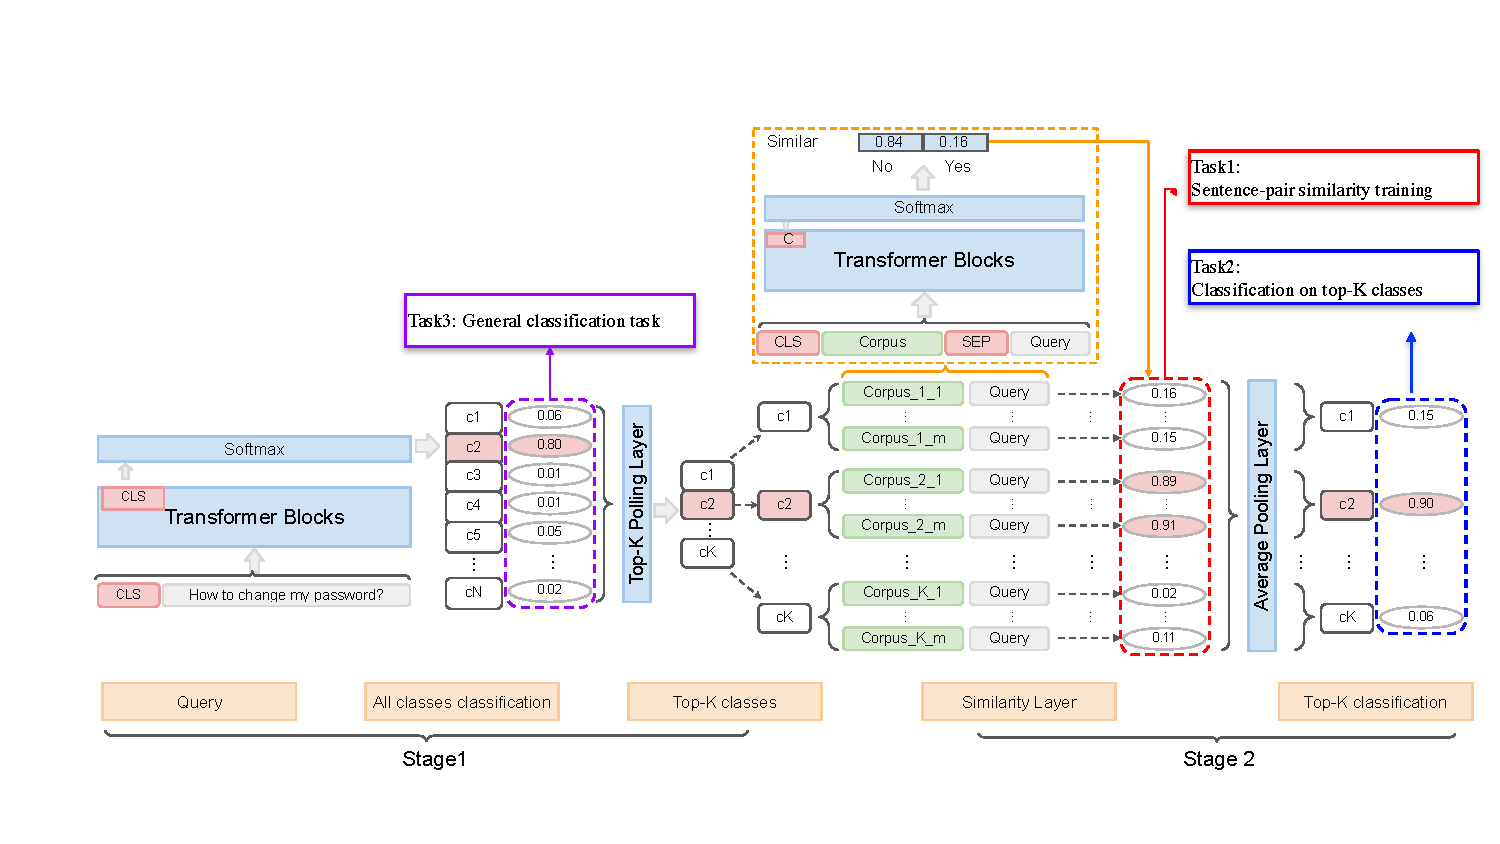
\includegraphics[scale=0.72]{picture/picture4} 
      \par
    \end{centering}
    \caption{
      \textbf{Network   Structure   of  joint  SFC:}  a  joint  model  of
      sentence-pair   model   and   text   classification   model  organized  in
      joint  structure by completing different tasks at different network
      layers.
    }
    \label{fig:framework}
  \end{figure*}

  \section{Methodology}
  In  this  section,  we  will  describe a system of similarity model fused with
  classification  model,  named  as  SFC, in detail. We come up with 2 different
  approaches  for  implementation  of SFC system, in which joint SFC is a
  further improvement of two-stage SFC for better performance.

  \subsection{two-stage SFC with multi-task learning}

  The   detailed   network   structure   of   two-stage   SFC  is  shown  in  Fig.
  \ref{fig:ver.1.3}.  It  is  composed  with  2  separate  stages  in  charge of
  different  jobs. In stage 1, we can use any auxiliary model or tool to provide
  top-K  most  related class labels for sampling sentence pairs of both positive
  samples  and negative samples for stage 2. Suppose we have a training data set
  $\mathcal{D}=\{x_{i},y_{i}\}_{i=1}^{N}$  of  $N$ data points, in which $x_{i}$
  is the user input query and $y_{i}$ is a single class label from a class label
  set  of  $C$  classes  in total. If we want to generate sentence pair data set
  $\mathcal{D'}=\{[(x,x')_{j},l_{j}]\}_{j=1}^{M}$,   where   $(x,   x')_{j}$  is
  sentence  pair  grouped  by  2  user  input  queries and $l_{j}\in\{0, 1\}$ is
  similarity class label, see Equ. \ref{eq:similarity label},
  \begin{align}
    l_{j}=
    \begin{cases} \label{eq:similarity label}
      0 & y_{x}\neq y_{x'}\\
      1 & y_{x}=y_{x'}
    \end{cases}
  \end{align}
  directly  from  original data set $\mathcal{D}$ without any sampling strategy,
  then  $\mathcal{D'}$  will  have  $M=N^2$ data points of sentence pairs, which
  might be too time-consuming for the training process of stage 2 since we often
  have  hundreds  of class labels under task-specific chatbot scenario. Although
  we  may  only  have  a  few data points for a single class label, $M$ is still
  quite a big number.

  Therefore,  we adopt the idea of adversarial negative sampling strategy raised
  by   \cite{bamler2020extreme}.  The  key  idea  of this sampling strategy is to
  train  with  negative  samples that are hard to be distinguished from positive
  samples. Now suppose we have a user input query $x_{i}$ and top-K most related
  class   labels   set  $\mathcal{C'}=\{c'_{1},  \dots,  c'_{K}\}$  provided  by
  auxiliary  model  or  tool in stage 1, where $K$ is a hyperparameter set by us
  that  controls  candidate  class  number,  we  apply  the adversarial negative
  sampling  strategy  into our sentence pair sampling process by the following 2
  steps:

  \textbf{1.  positive  sentence pair sampling}: During the training process, we
  have  to first make sure that the ground truth class label $y_{i}$ for $x_{i}$
  is  within  the  candidate  class  label  set  $\mathcal{C'}$. If $y_{i}\notin
  \mathcal{C'}$,  we  will manually add $y_{i}$ into $\mathcal{C'}$ by replacing
  $c'_{K}$  with  $y_{i}$, since $c'_{K}$ is the least promising candidate label
  according  to  the  auxiliary  model  in stage 1. Afterwards, we will randomly
  sample  $P$  sentences  $\{x'_{0},x'_{1}, \dots, x'_{P}\}$ with the same class
  label as $y_{i}$ from data set $\mathcal{D}$ to form the set of sentence pairs
  with   positive   label  $\mathcal{P'}_{i}=\{[(x_{i},  x'_{0}),  1],  [(x_{i},
  x'_{1}),   1],   \dots,   [(x_{i},   x'_{P}),  1]\}$,  where  $P$  is  also  a
  hyperparameter  set  by  us  that  controls  the number of sentences we should
  sample from each class.

  \textbf{2.  negative  sentence pair sampling}: As for negative sentence pairs,
  we  will  also  randomly  sample  $P$ sentences for each class in the negative
  candidate class label set $\mathcal{C'}\backslash \{y_{i}\}$. The class labels
  in  $\mathcal{C'}\backslash  \{y_{i}\}$  are  the  set of most confusing class
  labels comparing to the ground truth ${y_{i}}$, so we assume that the sentence
  pairs  with  negative  label grouped by user input query $x_{i}$ and sentences
  with class labels in $\mathcal{C'}\backslash \{y_{i}\}$ are strong adversarial
  negative  samples for sentence-pair similarity model that can help enhance the
  training  speed  and  performance.  According  to  the same method as positive
  sentence  pair sampling, we can obtain the set of sentence pairs with negative
  label  as $\mathcal{N'}_{i}=\{[(x_{i}, x'_{0}), 0], [(x_{i}, x'_{1}), 0], ...,
  [(x_{i}, x'_{P\cdot (K-1)}), 0]\}$

  In  this  way,  we  can generate the sentence pair data set $\mathcal{D'}$ for
  stage  2 based on the top-K class label set $\mathcal{C'}$ provided by stage 1
  as   $\mathcal{D'}=\{\mathcal{P'}_{i}\cup   \mathcal{N'}_{i}\}_{i=1}^{N}$,  in
  which we will have $M=N\cdot K\cdot P$ data points of sentence pairs in total.

  After  explaining the data sampling principle for sentence pairs and how the 2
  stages  in  SFC  system  connect  with  each other, let's go deeper into model
  structure within these two stages respectively to see how it works.

  \subsubsection*{
    stage 1: classification model for providing top-K candidate class labels
  }

  As for  stage  1,  our  SFC  system  can adapt to any auxiliary model or even
  searching  tool  based  on  Term Frequency-Inverse Document Frequency (TF-IDF)
  retrieval.  In  this  paper,  however,  we  choose to fine-tune RoBERTa on our
  task-specific  data set $\mathcal{D}$ by adding a softmax classifier on top of
  it,  the  same  as  the  structure shown in Fig. \ref{Fig.1.sub.1}, for better
  overall  performance.  According  to  our  experimental  result,  RoBERTa  can
  guarantee  that  approximately  95\%  ground  truth label be included in top-5
  candidate  class  labels  with  highest  probability after being fine-tuned on
  task-specific  data set with experimental result measured by F-score at around
  0.75.  So  we use RoBERTa as encoder of classification model in our setting at
  stage 1 to ensure low limitation for the performance of stage 2.

  For single-sentence text classification tasks, given a data point $x_{i}$ with
  class  label  $y_{i}$  from  data  set  $\mathcal{D}$, RoBERTa takes the final
  hidden  state  $h_{i}$  of the first token [CLS] as the representation for the
  whole   sequence  of  $x_{i}$.  Let's  suppose  we  have  a  linear  layer  as
  ${\Phi}^C_{i}=W^Ch_{i}+b^C$,  where  $W^C$ and $b^C$ are trainable parameters,
  the    probability    score    for    $x_{i}$    can    be    calculated    as
  $p^C_{i}=softmax(W^Ch_{i}+b^C)=softmax({\Phi}^C_{i})$.   Then,  the  loss  for
  stage 1 classification model is shown in Equ. \ref{eq:classification loss}, in
  which  the  first  term  $\varPhi_{i,y_{i}}^C$ encourages high probability for
  prediction of the correct label $y_{i}$.

  \begin{equation}
    \begin{aligned}
      \mathcal{L}^{C}&=\frac{1}{N}\sum_{i=1}^{N}-log(\frac{exp(\varPhi_{i,y_{i}}^C)}{\sum_{j=1}^{C}exp(\varPhi_{i,j}^C)}) \\&=\frac{1}{N}\sum_{i=1}^{N}-\varPhi_{i,y_{i}}^C+log(\sum_{j=1}^{C}exp(\varPhi_{i,j}^C))
      \label{eq:classification loss}
    \end{aligned}
  \end{equation}

  \subsubsection*{
    stage 2: sentence-pair model for multi-task learning
  }

  As for  stage 2, we also choose RoBERTa as the encoder for sentence pairs, as
  shown  in Fig. \ref{fig:ver.1.3}. Before sending sentence pairs to Roberta, we
  pack  sentence  pairs  into a single sequence and separate them with a special
  token  [SEP].  Roberta  will  also  add  a  learned  embedding  to every token
  indicating  whether  it belongs to the first sentence or the second one. Then,
  we  utilize  the  cross-attention  mechanism  inside RoBERTa, and then extract
  semantic relationship between 2 sentences from the output softmax layer, which
  is placed on top of the last hidden representation of the [CLS] token.

  Before we start to fine-tune our sentence-pair model on task-specific dataset,
  we   first  fine-tune  RoBERTa  on  Quora  dataset \cite{iyer2017first},  which
  contains  404,290  potential  duplicate question pairs, for transfer learning.
  Then   we   continue  to  do  multi-task  training  on  sentence-pair  dataset
  $\mathcal{D'}$ sampled from the top-K candidate class labels provided by stage
  1.

  The 2 tasks for stage 2 training process are listed below.

  $\bullet$ \textbf{Task 1: Regular sentence-pair similarity task}

  For  sentence  pair semantic similarity task, given a data point $(x, x')_{i}$
  with       similarity       label       $l_{i}$       from       data      set
  $\mathcal{D'}=\{[(x,x')_{i},l_{i}]\}_{i=1}^{M}$,   Roberta   takes  the  final
  hidden  state  $h_{i}$  of the first token [CLS] as the representation for the
  sequence of packed sentence pair $(x, x')_{i}$. Let's suppose we have a linear
  layer  as  ${\Phi}^S_{i}=W^Sh_{i}+b^S$,  where  $W^S$  and $b^S$ are trainable
  parameters,  and  the probability score for $(x, x')_{i}$ can be calculated as
  $p^S_{i}=softmax({\Phi}^S_{i})$.

  Due  to  the  fact that sentence pairs within the same class is much less than
  sentence  pairs  from  different  classes,  the  data  set  $\mathcal{D'}$  is
  imbalanced.  Therefore, we will accommodate a weight variable $w^S = [K-1, 1]$
  to  the  loss  to eliminate the bias brought by imbalanced data, shown in Equ.
  \ref{eq:similarity loss}.

  \begin{equation}
    \begin{aligned}
      \mathcal{L}^{S}&=\frac{1}{M}\sum_{i=1}^{M}-w^S_{l_i}\cdot log(\frac{exp(\varPhi_{i,l_{i}}^S)}{\sum_{j=0}^{1}exp(\varPhi_{i,j}^S)}) \\&=\frac{1}{M}\sum_{i=1}^{M}-w^S_{l_i}\cdot \varPhi_{i,l_{i}}^S+w^S_{l_i}\cdot log(\sum_{j=0}^{1}exp(\varPhi_{i,j}^S))
      \label{eq:similarity loss}
    \end{aligned}
  \end{equation}

  $\bullet$ \textbf{Task 2: Classification task on top-K classes based on sentence-pair model}

  As  for top-K classification task, it shares the same sentence-pair similarity
  model   structure  with  task  1.  The  only  difference  is  that  we  add  a
  task-specific  average  pooling  layer,  shown  in  Fig.  \ref{fig:ver.1.3} to
  implement the classification task based on sentence-pair model.

  We  already  know  that the size of ${\Phi}^S$ in task 1 is $M\times 2=(N\cdot
  K\cdot  P)\times  2$, where $N$ is the total number of data points in original
  training  data $\mathcal{D}$, $K$ is a hyperparameter that controls the number
  of   candidate   class  labels  provided  by  stage  1,  and  $P$  is  also  a
  hyperparameter that controls the number of sentences we should randomly sample
  from each candidate class labels. Now, for the average pooling layer, we first
  reshape  ${\Phi}^S$  into  the  size  of $N\times K\times P\times 2$, and then
  split  it  into  ${\Phi}^{K,pos}$  and ${\Phi}^{K,neg}$, and both of them will
  have  the  size  of  $N\times  K\times  P$.  In this way, ${\Phi}^{K,pos}$ can
  represent  the  level  of  similarity  for each sentence pair, and in the mean
  time,  ${\Phi}^{K,neg}$  can  represent  the  level  of dissimilarity for each
  sentence  pair. Then, we can do average pooling for each candidate class among
  the  top-K  classes  as  shown  in  Equ.  \ref{eq:average  pooling:1} and Equ.
  \ref{eq:average pooling:2}.

  \begin{align}
    {\xi}_{i,j}^{K,pos} = \sum_{p=1}^{P}{\varPhi}_{i,j,p}^{K,pos} \label{eq:average pooling:1}\\
    {\xi}_{i,j}^{K,neg} = \sum_{p=1}^{P}{\varPhi}_{i,j,p}^{K,neg}
    \label{eq:average pooling:2}
  \end{align}

  With  the  average pooling result ${\xi}^{K,pos}$ and ${\xi}^{K,neg}$, we also
  generate   a   top-K   class   label   $l^{K}_i\in   [1,\dots,K]$   for   each
  ${\xi}^{K,pos}_{i}$ and ${\xi}^{K,neg}_{i}$. The loss for top-K classification
  task is shown in Equ. \ref{eq:top-k classification loss}. In Equ. \ref{eq: pos
  top-k   loss}   and   Equ.   \ref{eq:   neg   top-k   loss},  the  first  term
  $\xi_{i,l^{K}_{i}}^{K,pos}$  and  $\xi_{i,l^{K}_{i}}^{K,neg}$  encourage  high
  level  of  similarity  and  low  level  of dissimilarity for prediction of the
  correct label $l^{K}_i$ within the top-K candidate classes.

  \begin{align}
    \mathcal{L}^{K} = \frac{1}{N}\sum_{i=1}^{N}(\mathcal{L}^{K,pos}_{i} - \mathcal{L}^{K,neg}_{i})
    \label{eq:top-k classification loss}
  \end{align}
  where,

  \begin{equation}
    \begin{aligned}
      \mathcal{L}^{K,pos}_{i} &= -log(\frac{exp(\xi_{i,l^{K}_{i}}^{K,pos})}{\sum_{j=1}^{K}exp(\xi_{i,j}^{K,pos})}) \\
      &= -\xi_{i,l^{K}_{i}}^{K,pos} + log(\sum_{j=1}^{K}exp(\xi_{i,j}^{K,pos}))
      \label{eq: pos top-k loss}
    \end{aligned}
  \end{equation}

  \begin{equation}
    \begin{aligned}
      \mathcal{L}^{K,neg}_{i} &= -log(\frac{exp(\xi_{i,l^{K}_{i}}^{K,neg})}{\sum_{j=1}^{K}exp(\xi_{i,j}^{K,neg})}) \\
      &= -\xi_{i,l^{K}_{i}}^{K,neg} + log(\sum_{j=1}^{K}exp(\xi_{i,j}^{K,neg}))
      \label{eq: neg top-k loss}
    \end{aligned}
  \end{equation}

  Therefore,  the  overall  loss  function for multi-task learning in stage 2 is
  shown in Equ. \ref{eq: two-stage SFC loss}. The training objective of stage 2 is
  to  minimize  the  weighted  sum  of task-specific losses. Here $\alpha_S$ and
  $\alpha_K$  are  weights  of  task  1  and  task  2  respectively,  which  are
  $\alpha_S=0.125$ and $\alpha_K=0.875$ in our setting.

  \begin{align}
    \mathcal{L} = \alpha_S \mathcal{L}^S + \alpha_K \mathcal{L}^K
    \label{eq: two-stage SFC loss}
  \end{align}

  \begin{table*}
    \begin{centering}

      \begin{tabular}{|c|c|c|c|c|c|}
        \hline 
        Dataset & Domain & \#Class & \#Samples & \#Samples/Class & Experimental Settings\tabularnewline
        \hline 
        ITG & FAQ chatbot & 228 & 3938 & 17 & 3-fold\tabularnewline
        \hline 
        Amazon-670k & Product review & 250 & 1942 & 8 & class sampling\tabularnewline
        \hline 
        HWU64 & Intent detection & 64 & [320, 640, 960, 1280] & [5, 10, 15, 20] & data sampling\tabularnewline
        \hline 
        CLINC150 & Intent detection & 150 & [750, 1500, 2250] & [5, 10, 15] & data sampling\tabularnewline
        \hline 
        BANKING77 & Intent detection & 77 & [385, 770, 1155, 1540] & [5, 10, 15, 20] & data sampling\tabularnewline
        \hline 
      \end{tabular}
      \par
    \end{centering}
    \caption{Key statistics for experimental datasets and few shot settings}

    \label{tbe:dataset statistic}
  \end{table*}

  \subsection{joint SFC with joint model structure}
  Despite  the  outstanding experimental result of two-stage SFC on various tasks,
  we still find a limitation brought by the two-stage system structure. In two-stage
  SFC, Stage 1 and stage 2 are separate, so they do not interact with each other
  during  training.  In  this  case,  the  performance  of stage 1 can limit the
  potential  of  stage  2, meanwhile, stage 2 also cannot give training feedback
  back to stage 1 for fine-tuning.

  Therefore,  to  further  improve the overall performance of SFC, we proposed a
  joint  model  structure,  shown  in Fig. \ref{fig:framework}. In
  joint SFC, classification model is being placed in lower layer level to
  dynamically  provide  top-K  candidate  class  labels  for  the  sentence-pair
  similarity  model  placed in higher layer level through a top-K pooling layer.
  In  this way, classification model and similarity model can be merged into one
  single  joint-model  for  multi-task training with sentence pairs sampled from
  varying  candidate  class  labels,  thus  avoiding the limitation brought by 2
  separate stage structure.

  There  are  3  tasks in total during the training process of joint SFC,
  shown  in  Fig. \ref{fig:framework}, and the overall loss is also the weighted
  sum  of  all  the task-specific losses, shown in Equ. \ref{eq: hierachical SFC
  loss}. Here, $\alpha_S$, $\alpha_K$ and $\alpha_C$ are the weights for task 1:
  sentence-pair  similarity,  task  2:  top-K classification and task 3: general
  single   sentence  classification  respectively,  which  are  $\alpha_S=0.25$,
  $\alpha_K=0.25$ and $\alpha_C=0.5$ in our setting.

  \begin{align}
    \mathcal{L} = \alpha_S \mathcal{L}^S + \alpha_K \mathcal{L}^K + \alpha_C \mathcal{L}^C
    \label{eq: hierachical SFC loss}
  \end{align}

  Finally,  when  doing inference, for each user input query $x$, we will choose
  the  class label that contains the sentence $x'$ with highest similarity score
  $\varPhi$,  after  being packed into a sentence pair $(x, x')$ with query $x$,
  as our final result for prediction.

  \section{Experiments}
  In  this  section,  we  conduct  extensive  experiments  over  5 task-specific
  datasets  to  evaluate  the  performance  of  our  proposed SFC system and the
  effectiveness  of  the  methodology  of  multi-task  learning  and hierachical
  joint-model structure under low-data settings.

  \subsection{Datasets}
  The  datasets  used in our experiments aims to help us study low-resource text
  classification  problem  under  task-specific conversational chatbot scenario.
  Therefore,  we keep all the dataset under low-resource chatbot corpus setting,
  which  is a large number of class labels (50-250) with a few examples(5-20) in
  short  text  for  each  class, by sampling smaller subsets from the full scale
  when the raw datasets are oversized, see Table \ref{tbe:dataset statistic}.

  According to the task and domain, we categorize our experimental datasets into
  the following 3 categories:

  $\bullet$ \textbf{Full-scale real-world task-specific faq chatbot dataset}

  \textbf{ITG}  is  a  real-world  FAQ  chatbot dataset composed of question and
  answer pairs about online English teaching. It contains 3,938 sample questions
  for  228  class labels, where each class label corresponds to an unique answer
  for a bunch of similar sample questions.

  We  divide the whole dataset into 3 folds randomly with approximately the same
  amount  of data within each fold, and then choose 2 folds as the training set,
  the  remaing  1  fold  as  the  test  set for our experiments. We can obtain 3
  different  combinations  among  the  3  folds,  and  we  will  use the average
  experimental  results  of  these 3 combinations as the final evaluation result
  for this dataset.

  $\bullet$ \textbf{Subset of customer review dataset for extreme classification}

  \textbf{Amazon-670K}   is   a   customer   product  review  dataset  for  text
  classification  task from the extreme classification repository with full data
  containing  670,091  class  labels,  285,176  training samples and 150875 test
  samples \cite{bhatia2016extreme}.  As  the  data  set  contains  multiple class
  labels  per  training sample, we keep only the first class label for each data
  point. Besides, we also randomly sampled 250 class labels from all the classes
  that  contain only 5-15 data points. In this way, we simulate the low-resource
  chatbot  corpus setting with the subset of 1,942 training samples and 716 test
  samples for 250 class labels.

  $\bullet$ \textbf{Subset of recently-released intent detection datasets}.

  From our point of view, task-specific chatbot usually starts with small amount
  of  data at the initial stage. As more and more customers start to communicate
  with  the  chatbot,  more data can be extracted from conversation log. Base on
  these  assumptions,  we  do  experiments  on  the following 3 intent detection
  dataset    under    sampling    method    similar    to    the   approach   in
   \cite{casanueva2020efficient}  but  in  more  sophisticated few-shot settings,
  while  keeping the same test sets for each experiment to see the change of the
  improvement scale with decreasing data amount.


  \begin{table*}
    \begin{centering}
      \scalebox{0.8}{
        \begin{tabular}{|c|ccc|cccc|cccc|c|c|}
          \hline 
          \multicolumn{1}{|c|}{\multirow{2}*{\textbf{Models}} }& \multicolumn{3}{c|}{\textbf{CLINC150}}& \multicolumn{4}{c|}{\textbf{BANKING77}}& \multicolumn{4}{c|}{\textbf{HWU64}}& \ \ \ \textbf{ITG} \ \ \ & \textbf{Amazon-670k}\tabularnewline
          \cline{2-14}
          \multicolumn{1}{|c|}{} & $\textbf{5}$ & $\textbf{10}$ & $\textbf{15}$ & $\textbf{5}$ & $\textbf{10}$ & $\textbf{15}$ & $\textbf{20}$ & $\textbf{5}$ & $\textbf{10}$ & $\textbf{15}$ & $\textbf{20}$ & \textbf{Full} & \textbf{Full}\tabularnewline
          \hline
          TextCNN & \multirow{2}*{$0.5318$} & \multirow{2}*{$0.6963$} & \multirow{2}*{$0.7609$} & \multirow{2}*{$0.4408$} & \multirow{2}*{$0.6436$} & \multirow{2}*{$0.7366$} & \multirow{2}*{$0.7918$} & \multirow{2}*{$0.3112$} & \multirow{2}*{$0.4007$} & \multirow{2}*{$0.4823$} & \multirow{2}*{$0.5272$} & \multirow{2}*{$0.6624$} & \multirow{2}*{$0.4401$}\tabularnewline
          (classification) & & & & & & & & & & & & &\tabularnewline
          \hline
          LEAM & \multirow{2}*{$0.7514$} & \multirow{2}*{$0.8203$} & \multirow{2}*{$0.8612$} & \multirow{2}*{$0.5422$} & \multirow{2}*{$0.7812$} & \multirow{2}*{$0.8129$} & \multirow{2}*{$0.8280$} & \multirow{2}*{$0.4545$} & \multirow{2}*{$0.5554$} & \multirow{2}*{$0.5936$} & \multirow{2}*{$0.6599$} & \multirow{2}*{$0.7086$} & \multirow{2}*{$0.6091$}\tabularnewline
          (classification) & & & & & & & & & & & & &\tabularnewline
          \hline
          BERT-large & \multirow{2}*{$0.8080$} & \multirow{2}*{$0.8904$} & \multirow{2}*{$0.9265$} & \multirow{2}*{$0.578$} & \multirow{2}*{$0.8004$} & \multirow{2}*{$0.8518$} & \multirow{2}*{$0.8827$} & \multirow{2}*{$0.4711$} & \multirow{2}*{$0.5963$} & \multirow{2}*{$0.6342$} & \multirow{2}*{$0.7010$} & \multirow{2}*{$0.7485$} & \multirow{2}*{$0.6658$}\tabularnewline
          (classification) & & & & & & & & & & & & &\tabularnewline
          \hline
          ALBERT-xxlarge & \multirow{2}*{$0.8497$} & \multirow{2}*{$0.9008$} & \multirow{2}*{$0.9296$} & \multirow{2}*{$0.5549$} & \multirow{2}*{$0.7981$} & \multirow{2}*{$0.8231$} & \multirow{2}*{$0.8530$} & \multirow{2}*{$0.4879$} & \multirow{2}*{$0.6116$} & \multirow{2}*{$0.6135$} & \multirow{2}*{$0.6996$} & \multirow{2}*{$0.7253$} & \multirow{2}*{$0.6893$}\tabularnewline
          (classification) & & & & & & & & & & & & &\tabularnewline
          \hline
          RoBERTa-base & \multirow{2}*{$0.8732$} & \multirow{2}*{$0.9254$} & \multirow{2}*{$0.9363$} & \multirow{2}*{$0.7305$} & \multirow{2}*{$0.8654$} & \multirow{2}*{$0.8808$} & \multirow{2}*{$0.9080$} & \multirow{2}*{$0.5831$} & \multirow{2}*{$0.6790$} & \multirow{2}*{$0.7064$} & \multirow{2}*{$0.7100$} & \multirow{2}*{$0.7734$} & \multirow{2}*{$0.6708$}\tabularnewline
          (classification) & & & & & & & & & & & & &\tabularnewline
          \hline
          RoBERTa-large & \multirow{2}*{$0.8974$} & \multirow{2}*{$0.9372$} & \multirow{2}*{$0.9508$} & \multirow{2}*{$0.7690$} & \multirow{2}*{$0.8728$} & \multirow{2}*{$0.8966$} & \multirow{2}*{$0.9099$} & \multirow{2}*{$0.6044$} & \multirow{2}*{$0.7002$} & \multirow{2}*{$0.7129$} & \multirow{2}*{$0.7436$} & \multirow{2}*{$0.7990$} & \multirow{2}*{$0.7156$}\tabularnewline
          (classification) & & & & & & & & & & & & &\tabularnewline
          \hline
          RoBERTa-large & \multirow{2}*{$0.8266$} & \multirow{2}*{$0.8861$} & \multirow{2}*{$0.9023$} & \multirow{2}*{$0.757$} & \multirow{2}*{$0.8476$} & \multirow{2}*{$0.8614$} & \multirow{2}*{$0.8743$} & \multirow{2}*{$0.5425$} & \multirow{2}*{$0.6164$} & \multirow{2}*{$0.6503$} & \multirow{2}*{$0.6729$} & \multirow{2}*{$0.7418$} & \multirow{2}*{$0.6362$}\tabularnewline
          (similarity) & & & & & & & & & & & & &\tabularnewline
          \hline
          two-stage SFC & \multirow{2}*{$0.8979$} & \multirow{2}*{$0.9457$} & \multirow{2}*{$0.9517$} & \multirow{2}*{$0.7975$} & \multirow{2}*{$0.8818$} & \multirow{2}*{$0.8962$} & \multirow{2}*{$0.9109$} & \multirow{2}*{$0.6477$} & \multirow{2}*{$0.7055$} & \multirow{2}*{$0.7200$} & \multirow{2}*{$0.7232$} & \multirow{2}*{$0.7972$} & \multirow{2}*{$0.7189$}\tabularnewline
          (task1 only) & & & & & & & & & & & & &\tabularnewline
          \hline
          two-stage SFC & \multirow{2}*{$0.9162$} & \multirow{2}*{$0.9424$} & \multirow{2}*{$0.9530$} & \multirow{2}*{$0.7997$} & \multirow{2}*{$0.8823$} & \multirow{2}*{$0.8945$} & \multirow{2}*{$0.9123$} & \multirow{2}*{$0.6498$} & \multirow{2}*{$0.6980$} & \multirow{2}*{$0.7202$} & \multirow{2}*{$0.7358$} & \multirow{2}*{$0.8020$} & \multirow{2}*{$0.7311$}\tabularnewline
          (task2 only) & & & & & & & & & & & & &\tabularnewline
          \hline
          two-stage SFC & \multirow{2}*{$0.9167$} & \multirow{2}*{$0.9456$} & \multirow{2}*{$0.9571$} & \multirow{2}*{$0.7954$} & \multirow{2}*{$0.8854$} & \multirow{2}*{$0.8931$} & \multirow{2}*{$0.9192$} & \multirow{2}*{$0.6525$} & \multirow{2}*{$0.7001$} & \multirow{2}*{$0.7168$} & \multirow{2}*{$0.7476$} & \multirow{2}*{$\textbf{0.8124}$} & \multirow{2}*{$0.7364$}\tabularnewline
          (task1 + task2) & & & & & & & & & & & & &\tabularnewline
          \hline
          \multirow{2}*{joint SFC} & \multirow{2}*{$\textbf{0.9231}$} & \multirow{2}*{$\textbf{0.9560}$} & \multirow{2}*{$\textbf{0.9644}$} & \multirow{2}*{$\textbf{0.8270}$} & \multirow{2}*{$\textbf{0.9069}$} & \multirow{2}*{$\textbf{0.9103}$} & \multirow{2}*{$\textbf{0.9209}$} & \multirow{2}*{$\textbf{0.6697}$} & \multirow{2}*{$\textbf{0.7211}$} & \multirow{2}*{$\textbf{0.7254}$} & \multirow{2}*{$\textbf{0.7497}$} & \multirow{2}*{$0.8114$} & \multirow{2}*{$\textbf{0.7445}$}\tabularnewline
          & & & & & & & & & & & & &\tabularnewline
          \hline
        \end{tabular}
      }
      \par
    \end{centering}
    \caption{
      F-scores  on five task-specific dataset for text classification in chatbot
      under low resource. For ITG, we keep the full dataset. For Amazon-670k, we
      randomly  sampled  250  classes  with  training sample numbers within 5-15
      samples  per  class.  For  CLINC150,  BANKING77,  HWU64, we set up various
      few-shot  settings  (5/10/15/20  samples per class) while keeping the test
      set  to  be  fixed. The highest scores for each data setting are marked in
      bold.
    }

    \label{tbe:table2}
  \end{table*}

  \textbf{HWU64}   is  a  intent  detection  dataset  designed  for  home  robot
  scenario \cite{liu2019benchmarking}.  It aims at the specific task of capturing
  the  intent  for  different  user  requests  to  home  robot  and  finding the
  corresponding answer. The raw dataset contains 25,716 data points for 64 class
  labels  through  crowdsourcing,  which  raises  much  more  data  than  common
  real-world  circumstances. Therefore, we experiment with the setups where only
  5,  10,  15  and 20 training data points are available for each class label by
  random sampling.

  \textbf{CLINC150}  is a dataset designed for task-oriented systems with 23,700
  queries  that  are  short  and unstructured for 150 intents, in the same style
  made  by real users through crowdsourcing \cite{larson2019evaluation}. Here, we
  sample 5, 10 and 15 training data points for each intent class label by random
  sampling for our experimental setup.

  \textbf{BANKING77}  is  a intent detection dataset for bank customer services.
  The    raw    dataset    contains    13,084   data   points   for   77   class
  labels \cite{casanueva2020efficient}.  Here,  we  sample 5, 10, 15, 20 training
  data  points  for  each  class  label  by random sampling for our experimental
  setup.


  \subsection{Baselines}
  We choose 3 groups of representative baselines:

  \textbf{Group  1:  single-task  classification  model.} This group of baseline
  models  are  based  on the network structure for classification model shown in
  \ref{Fig.1.sub.1}.   As   for   non-pretrained   neural   network,  we  choose
  TextCNN \cite{kim2014convolutional}  as  a  representative baseline. As for the
  pretrained  model,  we choose RoBERTa, BERT and ALBERT, all of which are among
  the  most  powerful pretrained models that achieve outstanding results in many
  NLP  tasks,  in  our  experimental  setting. Since we apply RoBERTa in our SFC
  system,   we   naturally  adopt  single-task  classification  model  based  on
  RoBERTa-large  and RoBERTa-base as our baseline models. Besides, we also adopt
  the       recently       released       baseline       pre-trained       model
  ALBERT-xxlarge \cite{lan2019albert}  for  comparison.  Since  we  use different
  few-shot   settings   from    \cite{casanueva2020efficient}  for  those  intent
  detection  datasets,  we also use BERT-large tuned on our few-shot settings as
  an essential reference for experimental results.


  \textbf{Group  2: single-task similarity model.} This group of baseline models
  are   based   on   network   structure   for   similarity   model   shown   in
  \ref{Fig.1.sub.2}. We choose RoBERTa-large for the pretrained model part as an
  powerful baseline. But during the evaluation step, we use elastic search to do
  a  rough  filter  for  candidate  sentence  pairs  to  guarantee  a reasonable
  inference time for each user query.

  \textbf{Group  3:  SFC  system with ablation study.} This group of baseline is
  based  on  the network structure of two-stage SFC shown in \ref{fig:ver.1.3}. We
  conduct  ablation study by introducing single task SFC system with only Task 1
  or  Task  2  to  investigate  the influence of each component within the total
  loss.

  \subsection{Implementation Details}
  For  our  SFC  system,  we  use RoBERTa-large as the pretrained model for both
  classification  task  and  sentence-pair similarity task. We further fine-tune
  our  SFC  system  on  task-specific  datasets with max sequence length of 128,
  learning  rate  of 1.5e-5 for RoBERTa-large pretrained model and learning rate
  of  5e-4  for  task-specific  layer  with polynomial decay and Adam optimizer.
  Also,  we  set  the  max number of the epoch to 100 and save the best model on
  validation  set based on test result in F-score. We also report the F-score as
  the main evaluation measure for all experimental results.

  For  the  experiments  in  Table  \ref{tbe:table2},  we  empirically  set  the
  hyperparameter  to  be  $K=5$  and  $P=10$  for  all  SFC  variants.  In Table
  \ref{tbe:table3},  we  conduct extensive experiments to see the performance of
  SFC system under various hyperparameter settings.

  \begin{table*}
    \begin{centering}

      \begin{tabular}{|c|c|c|c|c|c|c|}
        \hline 
        \multicolumn{1}{|c|}{\multirow{2}*{Dataset}}&\multicolumn{1}{c|}{\multirow{2}*{Model}}& $K=3$ & $K=5$ & $K=10$ & $K=15$ & $K=20$\tabularnewline
        \multicolumn{1}{|c|}{} & \multicolumn{1}{c|}{} & $P=20$ & $P=10$ & $P=5$ & $P=4$ & $P=3$\tabularnewline
        \hline
        \multicolumn{1}{|c|}{\multirow{2}*{ITG}}& two-stage SFC & $0.8034$ & $0.8124$ & $0.8008$ & $0.7967$ & $0.7934$\tabularnewline
        \cline{2-7}
        \multicolumn{1}{|c|}{} & joint SFC & $0.7986$ & $0.8114$ & $0.8010$ & $0.7972$ & $0.7918$\tabularnewline
        \hline
        \multicolumn{1}{|c|}{\multirow{2}*{Amazon-670k}}& two-stage SFC & $0.7278$ & $0.7364$ & $0.7366$ & $0.7328$ & $0.7204$\tabularnewline
        \cline{2-7}
        \multicolumn{1}{|c|}{} & joint SFC & $0.7334$ & $0.7445$ & $0.7516$ & $0.7344$ & $0.7373$\tabularnewline
        \hline
      \end{tabular}
      \par
    \end{centering}
    \caption{
      We  show the performance of SFC from different settings of hyperparameters
      for  $K$,  the candidate class number, and $P$, the sample number for each
      class.
    }

    \label{tbe:table3}
  \end{table*}

  \subsection{Result Analysis}

  Table  \ref{tbe:table2}  presents  the  results for each experimental data and
  model  set-up  in detail. The performance of each model is measured in F-score
  on the fixed test set for each data set. The overall performance of SFC system
  is  better  than  all  the  competitive  single-model  baseline models on five
  experimental   datasets.  This  observation  gives  us  a  general  idea  that
  classification model and similarity model can actually provide each other with
  complementary information, and combining them together into a joint system can
  effectively  enhance the overall capability based on richer extracted semantic
  information.  However  the  relative performance among all the variants of SFC
  also  seems  to  depend  on  some  specific  charateristic  of  each data set.
  Therefore,  we did the following more detailed analysis from several different
  aspect.

  \textbf{Comparison  among  SFC  variants.} First, we turn to compare among the
  four  SFC  variants shown in Table \ref{tbe:table2} to analyze the improvement
  brought  by  multi-task  and  joint-model  structure. We conduct
  ablation  experiments  to study the benefits brought by multi-task training by
  comparing multi-task two-stage SFC with single-task two-stage SFC. We can see from
  Table  \ref{tbe:table2}  that  two-stage  SFC  with  only  task 1 (sentence-pair
  similarity task) degrades by 0.65 percent on average and two-stage SFC with only
  task  2  (top-K  classification  task) degrades by 0.32 percent on average. The
  degradation  indicates  that  training  with these 2 tasks together in SFC can
  effectively  help  the  sentence-pair  model  extract  more knowledge from the
  limited  amount  of data. Besides, task 2 degrades 0.33 percent less than task
  1.  This observation suggests that task 2 may play a relatively more important
  role  in multi-task learning, which leads us to put larger weight $\alpha_{K}$
  to  the  loss  $\mathcal{L}^{K}$  of  task  2  when calculating the total loss
  $\mathcal{L}$.  Also, we can see that the joint SFC steadily outperforms
  two-stage  SFC  on  5  diverse  datasets  by  1.17  percents  on  average.  This
  observation  supports  the idea that the joint model structure can
  alleviate the limitation brought by the lack of interaction between similarity
  model  and  classification  model in two-stage SFC. Therefore, for the following
  analysis,  we  will  focus  on  the comparison between joint SFC and the
  other baseline models.

  \textbf{Analysis  under  few-shot  scenarios.}  Next,  we  analyze the overall
  improvement trend of SFC under various few-shot settings. Our main focus is to
  study chatbot building in common situation during real-world application where
  only  a  few  sample  sentences are available for each class. The experimental
  results  for  the  3  diverse  intent detection datasets (ClINC150, BANKING77,
  HWU64) under few-shot settings indicate that our proposed joint SFC can
  achieve  2.47  percents  average  improvement  over  one  of the most powerful
  baseline  models,  which  is  RoBERTa-large classification model, on all these
  few-shot  settings. Moreover, the improvement in F-score becomes more and more
  prominent  with the decrease of data sample number per class. Our joint
  SFC   can  achieve  4.97  percents  average  improvements  over  RoBERTa-large
  classification model in the most extreme few-shot setting with only 5 training
  samples  per class. This observation indicates that SFC is especially suitable
  for  being  applied during the initial stage of building task-specific chatbot
  system,  where  the  amount  of  data sample for each class label is extremely
  scarce.

  \textbf{Comparison  between  label  embedding  and  sentence  pair embedding.}
  Afterwards,  we  start  to  compare the performance of SFC with the text-label
  joint  embedding  baseline  named as LEAM. As shown in Table \ref{tbe:table2},
  joint  SFC outperforms LEAM by 14.25 percents on average F-score over 5
  datasets.  Besides,  although the labels within the 3 diverse intent detection
  datasets  (CLINC150,  BANKING77,  HWU64)  are  all  being  well-defined as the
  semantic  summary  of  each intent, joint SFC still outperforms LEAM by
  14.69  percents  on  average  F-score.  This  observation  indicates that it's
  usually  quite  hard  to  use  a  fixed  label  with  only  a few words as the
  representative  of  all  the  sentences  within a class since there are always
  plenty of ways for people to express questions or queries about the same topic
  during   a   conversation  with  chatbot.  Therefore,  learning  the  semantic
  similarity  between  user  query  and  sample  sentences through sentence pair
  embedding  can be more reliable than making decision according to the semantic
  relationship between user query and class labels through label embedding.

  \textbf{Fusion  of  classification  and  similarity  model.} Then, we begin to
  compare  the  general  performance  of SFC with single-task classification and
  similarity  baselines.  As  for  the  classification  model,  joint SFC
  outperforms    TextCNN    by   26.19   percents,   ALBERT-xxlarge   by   9.95
  percents\footnote{We found that the performance of ALBERT.xxlarge is extremely
  unstable  for  classification  task.  Here, we did multiple run with different
  settings  of parameters such as learning rate and batch size for each dataset,
  and  record  the  best  result  we  can  obtain  in  Table \ref{tbe:table2}.},
  BERT-large  by  9.81 percents, RoBERTa-base by 4.52 percents, RoBERTa-large by
  2.47 percents on average F-score over 5 datasets. In this way, we can see that
  RoBERTa  is  the  best  baseline  pre-trained  model for the low-resource text
  classification  task  we  are  studying.  As for the similarity model, we only
  choose  the  strongest  pretrained  model  RoBERTa-large  as our baseline, and
  joint  SFC  achieves  the  improvement  of  7.81  percents  on average.
  Moreover,  joint  SFC's  result on 2 datasets without data sampling for
  few-shot  settings,  which  are  ITG  and  Amazon-670k, are also 1.24 and 2.89
  percents  higher  than  Roberta-large  classification  model, and are 6.96 and
  10.77  percents higher than Roberta-large similarity model. These improvements
  illustrate that putting classification model and similarity model at different
  network  layers  to  cooperate  with  each  other  is  a  successful design of
  joint network structure for joint model, which enables these two models
  assist each other for better overall results.

  \textbf{Settings  of  hyperparameters.} Finally, we analyze the effect brought
  by  different  settings  of  hyperparameters,  see  Table \ref{tbe:table3}. We
  conduct  experiments on 5 different settings of hyperparameters, which are the
  number  of candidate class number $K$ and the number of sentence pairs $P$ for
  each  class, on ITG and Amazon-670K datasets to find the most suitable setting
  of  these  2  hyperparameters.  We  control the total number of sentence pairs
  sampled  for  each  user  query  into  about  the same level of amount(50-60).
  Through  analyzing the experimenal results shown in Table \ref{tbe:table3}, we
  find  that the best setting of hyperparameters might be slightly different for
  datasets of different data size. The class label number of ITG and Amazon-670k
  are  similar  in  our  experimental  setting, which is around 250. However the
  total  amount  of  data  points  of  ITG  is approximately 2 times larger than
  Amazon-670k. Therefore, the setting of $K=5$ and $P=10$ is good enough for ITG
  since  most  of  the  classes  contains  over  10  data  points.  However, for
  Amazon-670k,  the amount of data sample for each class is scarce, thus, we may
  need  more  candidate  classes  to  sample enough effective sentence pairs for
  sentence-pair model layer of SFC. In this way, the setting of $K=10$ and $P=5$
  becomes a good choice. However, in spite of the effect on evaluation performance brought by different settings of hyperparameters, joint SFC still steadily outperforms two-stage SFC by 0.41 percents in overall average F-score on ITG and Amazon-670k datasets. 

  In  conclusion,  to  the best of our knowledge, these experimental results place joint SFC as the
  best   performing   model   on   5  diverse  experimental  datasets  for  text
  classification  task  under  low-resource task-specific conversational chatbot
  scenario.

  \section{Conclusion}
  In  this  work, we successfully proposed SFC, a joint system of classification
  model  and  sentence-pair similarity model with multi-task learning, which can
  effectively  alleviate  the  limitation of classification model and similarity
  model   for  low-resource  text  classification  tasks.  Experimental  results
  illustrate that our proposed system can achieve great improvement on 5 diverse
  datasets for task-specific chatbot system over several competitive single-task
  baseline  models. Furthermore, we especially analyze the excellent performance
  of SFC when facing the challenge brought by few-shot scenarios, which is quite
  common in real-world application of chatbot system.

  \bibliographystyle{aaai21}
  \bibliography{refs}

\end{document}
